\chapter{Simulation results}
\label{chap:simulation}

In this chapter, I simulate the matching process of a labor market, using real
data on workers' and firms' characteristics and assigned model parameters. I
then apply the two-sided logit model to show that the model is able to recover
the underlying parameters and to diagnose the properties of the MCMC sampling. I
compare the results of the two-sided logit model with the one-sided conditional
logit model, showing that the one-sided approach produces biased estimates of
workers' and firms' preference. This result demonstrates how the one-sided
approach, despite being the default method for analyzing two-sided markets, can
be misleading and unable to disentangle the effect of one side's preference from
the other's.

In addition, I explore the implications of the fact that, our FDI data does not
include the ``reservation choice,'' i.e. the choice that is always available.
Indeed, while labor market data often include unemployment as the reservation
choice, FDI data does not include firms who consider investing abroad but end up
staying home. Simulation results show that some of our estimates will be biased,
and I discuss potential remedies.

\section{Labor market data}

To ensure that my simulation result generalizes to real situations, I use real
data on workers' and firms' characteristics from the US General Social Survey
(GSS), 1982-1990.\footnote{I thank Professor Michael Newton and Professor John
  Allen Logan for sharing the dataset.} On one side of the matching market is
2149 workers, a representative sample of US male workers between 25 and 44 years
old. Table~\ref{tab:labor_occ5_summary_employee} shows the summary statistics
for these workers. On average, a worker is 33 ($\pm$ 5.7) years old and has 13
years ($\pm$ 3.1) of education. 11\% of workers in our sample are non-white.

\begin{table}[!ht]
  \centering
  \caption[Summary statistics of US male workers between 25 and 44 years old,
  1982-1990.]{Summary statistics of workers' education, age, and race. The data
    come from the GSS, 1982-1990, for male workers in the US between 25 and 44
    years old.}
  \label{tab:labor_occ5_summary_employee}
  
% Table created by stargazer v.5.2 by Marek Hlavac, Harvard University. E-mail: hlavac at fas.harvard.edu
% Date and time: Mon, Apr 02, 2018 - 13:50:38
\begin{tabular}{@{\extracolsep{5pt}}lccccc} 
\\[-1.8ex]\hline 
\hline \\[-1.8ex] 
Statistic & \multicolumn{1}{c}{N} & \multicolumn{1}{c}{Mean} & \multicolumn{1}{c}{St. Dev.} & \multicolumn{1}{c}{Min} & \multicolumn{1}{c}{Max} \\ 
\hline \\[-1.8ex] 
Years of education & 2,149 & 13.103 & 3.111 & 2 & 20 \\ 
Age & 2,149 & 33.524 & 5.716 & 25 & 44 \\ 
Non-white & 2,149 & 0.113 & 0.316 & 0 & 1 \\ 
\hline \\[-1.8ex] 
\end{tabular} 

\end{table}

On the other side of the matching market are five firms, representing five job
categories: professional, managerial, sales-clerical-services, manufacturing
blue collar, and other blue collar. Table~\ref{tab:labor_occ5_summary_employer}
shows their characteristics and the sub-categories from which they are
aggregated. \textit{Prestige} is the Hodge-Seigel-Rossi score, used in the GSS
to measure the prestige of a job \citep{Hodge1964, NORC2014}. \textit{Autonomy}
is calculated as the odds of having a supervisor, multiplied by -1 so that a
higher score is associated with a higher level of autonomy.\footnote{In other
  words, $\text{autonomy} = -\frac{P(\text{having a supervisor})}{P(\text{not
      having a supervisor})}$} The prestige and the autonomy scores of a firm in
our dataset are the average scores reported by workers who currently work in
that job categories. Unemployment by itself does not have a score. Following
\citet{Logan1996}'s study on the labor market, I set unemployment's prestige
score to 50\% of the prestige of the last job held and its autonomy score as the
average autonomy scores of all workers.

\begin{table}[tbp]
  \centering
  \caption[Characteristics of five firm types in the US,
  1982-1990.]{Characteristics of five firm types in the US, 1982-1990.}
  \label{tab:labor_occ5_summary_employer}
  
% Table created by stargazer v.5.2 by Marek Hlavac, Harvard University. E-mail: hlavac at fas.harvard.edu
% Date and time: Mon, Apr 02, 2018 - 13:50:38
\begin{tabular}{@{\extracolsep{5pt}} lccc} 
\\[-1.8ex]\hline 
\hline \\[-1.8ex] 
Firm category & Prestige & Pr(Supervisor) & Autonomy \\ 
\hline \\[-1.8ex] 
Unemployment & $18$ & $0.204$ & $$-$0.256$ \\ 
Professional & $59.670$ & $0.163$ & $$-$0.483$ \\ 
Managerial & $48.141$ & $0.442$ & $$-$3.237$ \\ 
Sales, Clerical, Services & $34.545$ & $0.100$ & $$-$0.112$ \\ 
Manufacturing Blue Collar & $34.330$ & $0.071$ & $$-$0.077$ \\ 
Other Blue Collar & $34.035$ & $0.175$ & $$-$0.214$ \\ 
\hline \\[-1.8ex] 
\end{tabular} 

\end{table}

\section{Simulated matching process}

I assign values to workers' and firms' preference parameters, choosing values to
achieve some level of realism and to have some workers in each job.
Table~\ref{tab:sim_labor_nojobs_utility_functions} describes the utility
functions. I normalize firms' utility of not hiring to 0 so that firm $j$ will
extend an offer to worker $i$ if the utility of hiring is positive (i.e.
$U_{j}(i) > 0$). The magnitude of the intercept can thus be interpreted as how
selective a firm is in making an offer. For example, professional and managerial
firms are highly selective with intercepts of $-24$ and $-22$, while the other
firms are less so with intercepts of $-9, -8$ and $-6$. The coefficients
represent how much a firm values a worker's trait. For example, managerial and
professional firms have a similar preference for a worker's education, with
coefficients of 1 and 1.3. On the other hand, managerial firm values a worker's
age twice as much as professional firm does, with coefficients of 0.2 and 0.1.

While the two-sided logit model can be extended to accommodate different worker
types as well, for this simulation I assume that workers have homogeneous
preference, sharing one utility function.

Each utility function has a random component, represented by the
Gumbel-distributed error term $\epsilon$. While normally distributed error is
more common in simulations, justified by the claim that the error term is the
sum of many independent unobserved variables, here I use the Gumbel distribution
so that the coefficient estimates from the two-sided logit model can be directly
compared with the true preference parameter values.\footnote{If I use normally
  distributed error terms, the coefficient estimates have to be divided by
  $\frac{\pi^2}{3}$ to be comparable with the true values. See \citet[chap
  2]{Train2009} for a more in-depth discussion of scaling and normalization in
  discrete choice models.} Practically the Gumbel distribution is very similar
to the normal distribution, and I discussed the implication of using the Gumbel
distribution in further depth in Section~\ref{sec:model_firm_decision_making}.

\begin{table}[!ht]
  \centering
  \caption[Utility functions used in labor market simulations.]{Utility
    functions of firms and workers used in labor market simulation. $x_{i1},
    x_{i2}, x_{i3}$ are worker \textit{i}'s education, age, and race (nonwhite
    is coded as 1). $w_{j1}, w_{j2}$ are firm \textit{j}'s prestige and
    autonomy, with $j \in \{1, \dots, 5\}$. The $\epsilon$'s are
    Gumbel-distributed error terms.}
  \label{tab:sim_labor_nojobs_utility_functions}
  \begin{tabular}{lll}
    \\[-1.8ex]\hline
    \textbf{Firms' utility functions}  &                                                                                     \\
    Professional                         & $U_{1}(i) = -24 + 1.3 x_{i1} + 0.1 x_{i2} + 1 x_{i3} + \epsilon$         \\
    Managerial                           & $U_{2}(i) = -22 + 1 x_{i1} + 0.2 x_{i2} + 1 x_{i3} + \epsilon$     \\
    Sales, Clerical, Services            & $U_{3}(i) = -9 + 0.75 x_{i1} + -0.05 x_{i2} + 0 x_{i3} + \epsilon$ \\
    Manufacturing blue collar            & $U_{4}(i) = -8 + 0.5 x_{i1} + 0.02 x_{i2} + 0 x_{i3} + \epsilon$   \\
    Other blue collar                    & $U_{5}(i) = -6 + 0.5 x_{i1} - 0.01 x_{i2} + 1 x_{i3} + \epsilon$   \\
    \hline
    \textbf{Workers' utility function} & $V_{i}(j) = 0.01 w_{j1} + 0.1 w_{j2} + \epsilon$                   \\
    \hline
  \end{tabular}
\end{table}

With these utility functions, I simulate the matching process as follows:

\begin{itemize}
\item{First stage:} Each firm $j$ evaluates each worker $i$, calculating the
  utility of hiring. If the utility of hiring is positive, it will extend an
  offer. Unemployment is always an option for workers, and is thought of as a
  ``firm'' that extends an offer to every worker. After this stage, we generate
  an opportunity set $O$ that is a $2149 \times 6$ matrix. In this matrix, cell
  $O_{ij}$ is 1 if worker $i$ receives an offer from firm $j$, and 0 if not. We
  typically do not observe this opportunity set matrix in real datasets.
\item{Second stage:} Worker $i$ evaluates each firm that extends him an offer in
  the first stage, calculating the utility of working for that firm. Worker $i$
  then chooses a firm (or unemployment) if it offers the highest utility. After
  this stage, we generate a choice vector that is a $2149 \times 1$ vector. In
  this choice vector, cell $i$ equals $j$ if worker $i$ decides to work at firm
  $j$. This choice vector is what we observe in real datasets such as the GSS.
\end{itemize}

\section{Simulation results}

I estimate the two-sided logit model using the MCMC approach described in
Chapter~\ref{chap:model}. For all preference parameters, I use a diffuse prior
that is a Normal distribution with mean 0 and variance 100. To propose new samples in the
Metropolis-Hastings algorithm, I use Normal distributions with a scale
hand-picked by examining the trace plots of discarded runs. The results below
are from a MCMC chain of 50,000 iterations with a thinning interval of 5,
resulting in 10,000 saved iterations.

Figure~\ref{fig:sim_labor_nojobs_alpha} shows the trace plots of the MCMC
samples for workers' preference. We see that the MCMC chain mixes well and
quickly converge to the true value indicated by the red line. This result gives
us confidence that the MCMC algorithm is implemented correctly and can achieve
convergence within a reasonable time frame.

\begin{figure}[!ht]
  \centering
  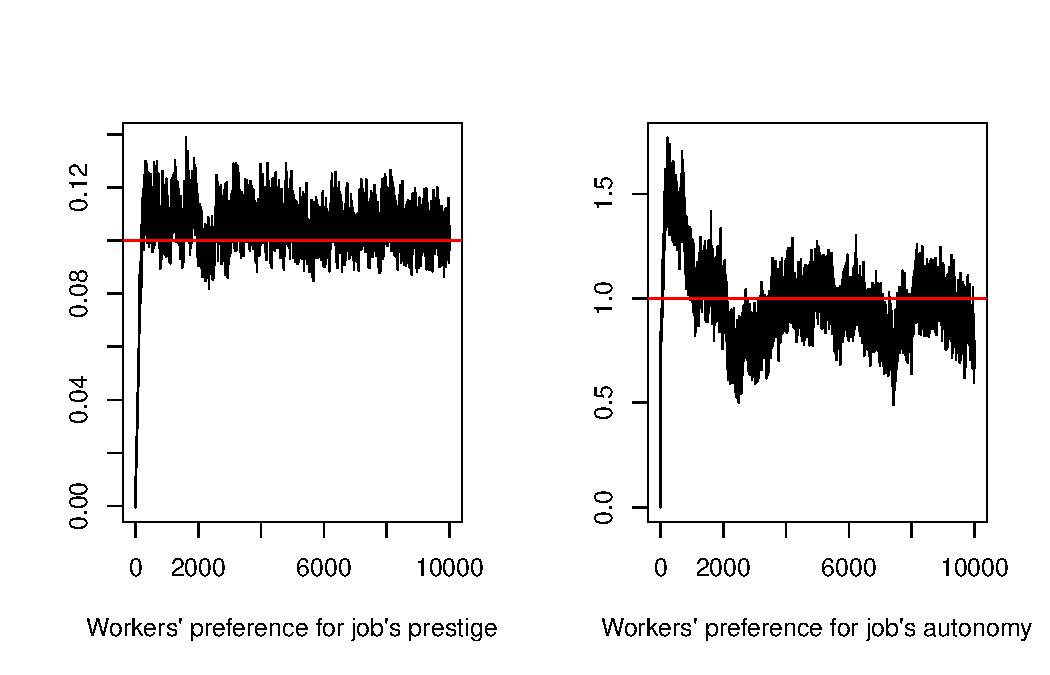
\includegraphics[width=\textwidth,keepaspectratio]{../figure/sim_labor_nojobs_alpha}
  \caption[Estimates for workers' preference]{Two-sided logit
    estimates for workers' preference. The black line plots are the trace plots
    of the MCMC samplers, and the red line indicates the true parameter values.
    The trace plots show that the MCMC chain is able to converge to the true
    value after 10,000 iterations (2,000 saved iterations $\times 5$ thinning
    interval).}
  \label{fig:sim_labor_nojobs_alpha}
\end{figure}

Figure~\ref{fig:sim_labor_nojobs_beta_emp2} shows the trace plots of the MCMC
samples for professional firm's preference. We see that the MCMC chain is also
able to converge to the true parameter values, albeit slower and with more
autocorrelation between iterations.\footnote{To improve the mixing of the MCMC
  chain, I standardize workers' characteristics so that they have mean 0.
  Therefore, the intercept term has to be changed accordingly. The true
  intercept values displayed in the plots are the standardized intercepts, which
  is different from those reported in
  Table~\ref{tab:sim_labor_nojobs_utility_functions}.} There are several reasons
for this poorer mixing.

\begin{figure}[tbp]
  \centering
  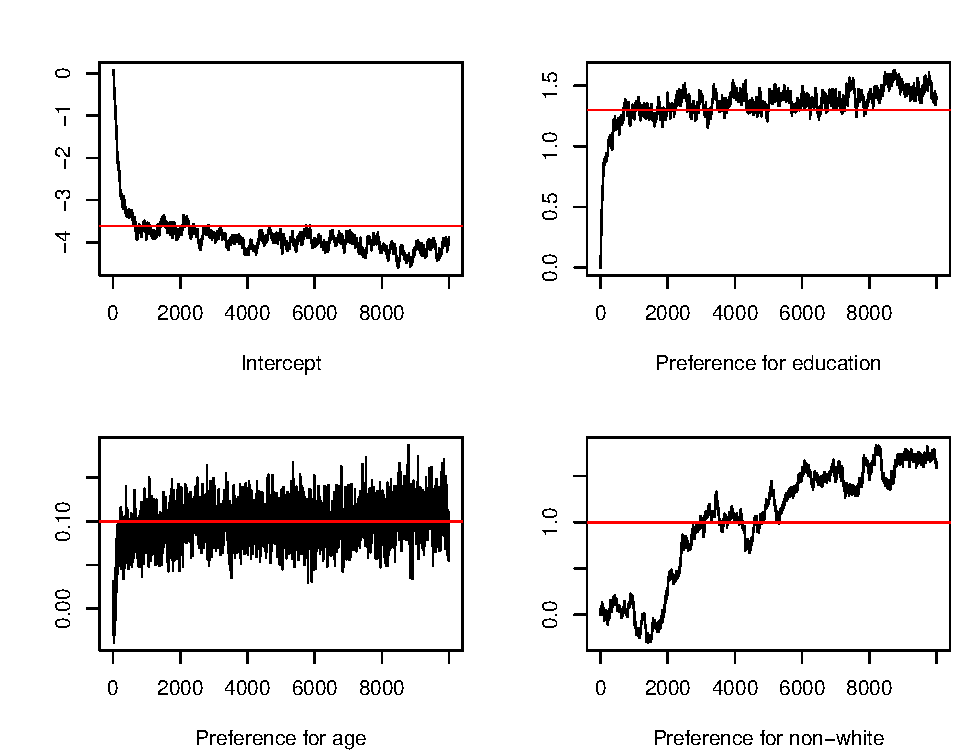
\includegraphics[width=\textwidth,keepaspectratio]{../figure/sim_labor_nojobs_beta_emp2}
  \caption[Estimates for professional firm's preference.]{Two-sided
    logit estimates for professional firm's preference. The MCMC chain is able
    to converge to the true parameter value, indicated by the red line, albeit
    with more autocorrelation than the MCMC chain for worker's preference in
    Figure~\ref{fig:sim_labor_nojobs_alpha}.}
  \label{fig:sim_labor_nojobs_beta_emp2}
\end{figure}

First, while we can use the entire sample to estimate the preference of workers,
only a subset of the sample works at a particular firm, resulting in a smaller
sample that we can use to estimate each firm's preference. This problem is
clearest in the trace plots for the managerial employer, which only has a sample
of 40 workers, or 1.9\% of the total sample \. To partially combat this issue, I
use a hierarchical model in which firms' preference parameters are drawn from a
common distribution. By doing so, I ``partially pool'' the sample across firms,
pulling the estimate for firms with small sample sizes towards the common mean,
and thus producing estimates that have more predictive power \citep{Gelman2006}.
For a similar reason, the MCMC chain of the preference parameter for
\textit{non-white} has a particularly poor mixing, likely because
\textit{non-white} is a binary variable, having less variation and thus
information that our model can use.

\begin{figure}[tbp]
  \centering
  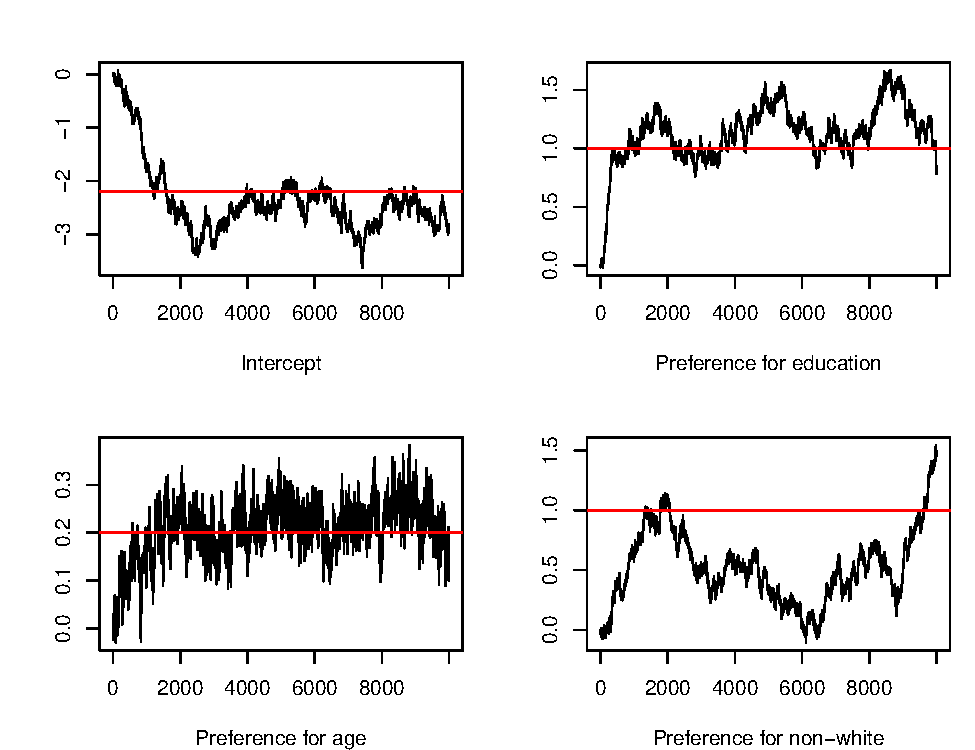
\includegraphics[width=\textwidth,keepaspectratio]{../figure/sim_labor_nojobs_beta_emp3}
  \caption[Poor mixing due to small sample size.]{Two-sided logit
    estimates for managerial firm's preference. Because the managerial firm only
    has a small sample size of 40 workers, or 1.9\% of the total sample, its
    preference is estimated more poorly than other's.}
  \label{fig:sim_labor_nojobs_beta_emp3}
\end{figure}

Second, while workers only have two preference parameters (for firm's prestige
and autonomy), each firm has four preference parameters (for worker's education,
age, race, and an intercept term), resulting in a total of 24 parameters.
Updating the MCMC chain in such high dimension is inherently difficult---to
update one parameter we only need to come up with one good proposal, but to
update 24 parameters we need to come up with good proposals for each of them.

Third, while firms' preference and the opportunity set are highly correlated,
our proposals for these parameters are independent, not take into their
correlation, and thus causing the MCMC to get stuck at local modes.
Section~\ref{sec:simulation_beta_opp_correlation} will discuss this issue and
potential remedies in more details.

\section{Comparing two-sided logit model and one-sided models}

In this section, I demonstrate that, without taking into account the two-sided
nature of the matching market, one-sided models produce biased estimates of the
actors' preference. While it may be unsurprising that one-sided models fail when
the data generating process is so different from their assumptions, this is a
worthwhile exercise given that many empirical researches rely on these models.
For example, using discrete choice models (multinomial logit, conditional
logit), \citet{Cheng2006} models Japanese MNCs' location choice across Chinese
provinces, \citet{Aw2008} models Taiwanese firms' decision to stay home or to
open a factory in China and the US.\footnote{In the empirical literature,
  researchers often use the term ``multinomial logit'' and ``conditional logit''
  interchangeably to refer to a discrete choice model of unordered choices. In
  this discussion, I follow the terminology in \citet{McFadden1974}'s seminal
  paper on discrete choice models, distinguishing ``multinomial logit'' as the
  model whose independent variables are the choosers' characteristics, and
  ``conditional logit'' as the model whose independent variables are the
  choices' characteristics.} Using count models (Poisson, negative binomial),
\citet{Wu1999} models MNCs' location choice in Guangzhou, China.
\citet{Arauzo-Carod2010} provides a literature review of how these one-sided
models are used in studying the location choice of firms.

Imitating these approaches in the literature, I estimate a conditional logit
model in which workers choose the best firm to work for as if all firms were
available in their opportunity set.
Figure~\ref{fig:sim_labor_nojobs_alpha_tsl_vs_cl} shows that the one-sided
conditional logit model produces biased estimates of workers' preference. Worse
yet, its estimate has little uncertainty and can cause researchers to be overly
confident in the wrong result.\footnote{This conditional logit model is
  equivalent to a Poisson model in which the dependent variable is the count of
  workers at each firm, as shown in \citet{Guimaraes2003}. Both models,
  estimated with MLE, would produce exactly the same estimates for the
  coefficients and their covariance matrix. Therefore, the argument against
  one-sided conditional logit applies fully to Poisson.}

\begin{figure}[tbp]
  \centering
  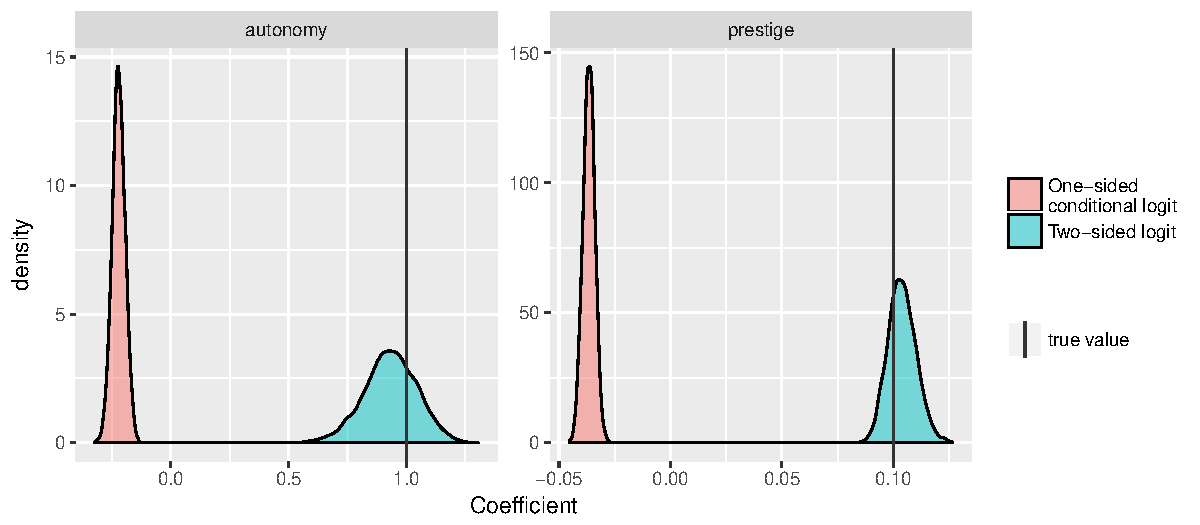
\includegraphics[width=\textwidth,keepaspectratio]{../figure/sim_labor_nojobs_alpha_tsl_vs_cl}
  \caption[Comparing two-sided logit's and one-sided
  conditional logit's estimates.]{Estimates of workers' preference, produced by
    two-sided logit and conditional logit. The density plots show that the
    two-sided logit's 95\% credible interval includes the true value, indicated
    by the black line, while the conditional logit's 95\% confidence interval is
    far from it.}
  \label{fig:sim_labor_nojobs_alpha_tsl_vs_cl}
\end{figure}

It is informative to examine the big difference between the two-sided and
one-sided estimates for \textit{prestige}. The reason for the large bias is
because the one-sided approach confounds the effect of one side's preference
with the other's. Figure~\ref{fig:sim_labor_nojobs_trueopp_obschoice} (left)
shows the binary heat map for the true opportunity set---a dark blue cell
indicates that an offer is made by firm in column $j$ to worker in row $i$. The
columns for professional and managerial firms (2\textsuperscript{nd} and
3\textsuperscript{rd} columns) are quite similar, reflecting the fact that they
have similar utility functions and make offers to the same kind of workers. In
contrast, in the observed choice
(Figure~\ref{fig:sim_labor_nojobs_trueopp_obschoice}, right), the columns for
professional and managerial firms are very different, reflecting the fact that
the professional firm is slightly more desirable, causing workers that receive
offers from both firms to overwhelmingly choose to work for the professional
firm over the managerial firm. Therefore, there are very few workers at the
managerial firm. To the one-sided conditional logit model, it looks as if the
managerial firm---a highly prestigious job---were less desirable than even the
services and blue collar firms. Therefore, it severely underestimate workers'
preference for \textit{prestige} to such an extent that \textit{prestige} is
considered a negative trait.

This example shows how misleading it can be to estimate workers' preference by
assuming that all the choices are available. Indeed, the managerial firm is
rarely chosen not because it is undesirable, but because it has to compete with
the professional firm for the same pool of highly educated and experienced
workers.

\begin{figure}[tbp]
  \centering
  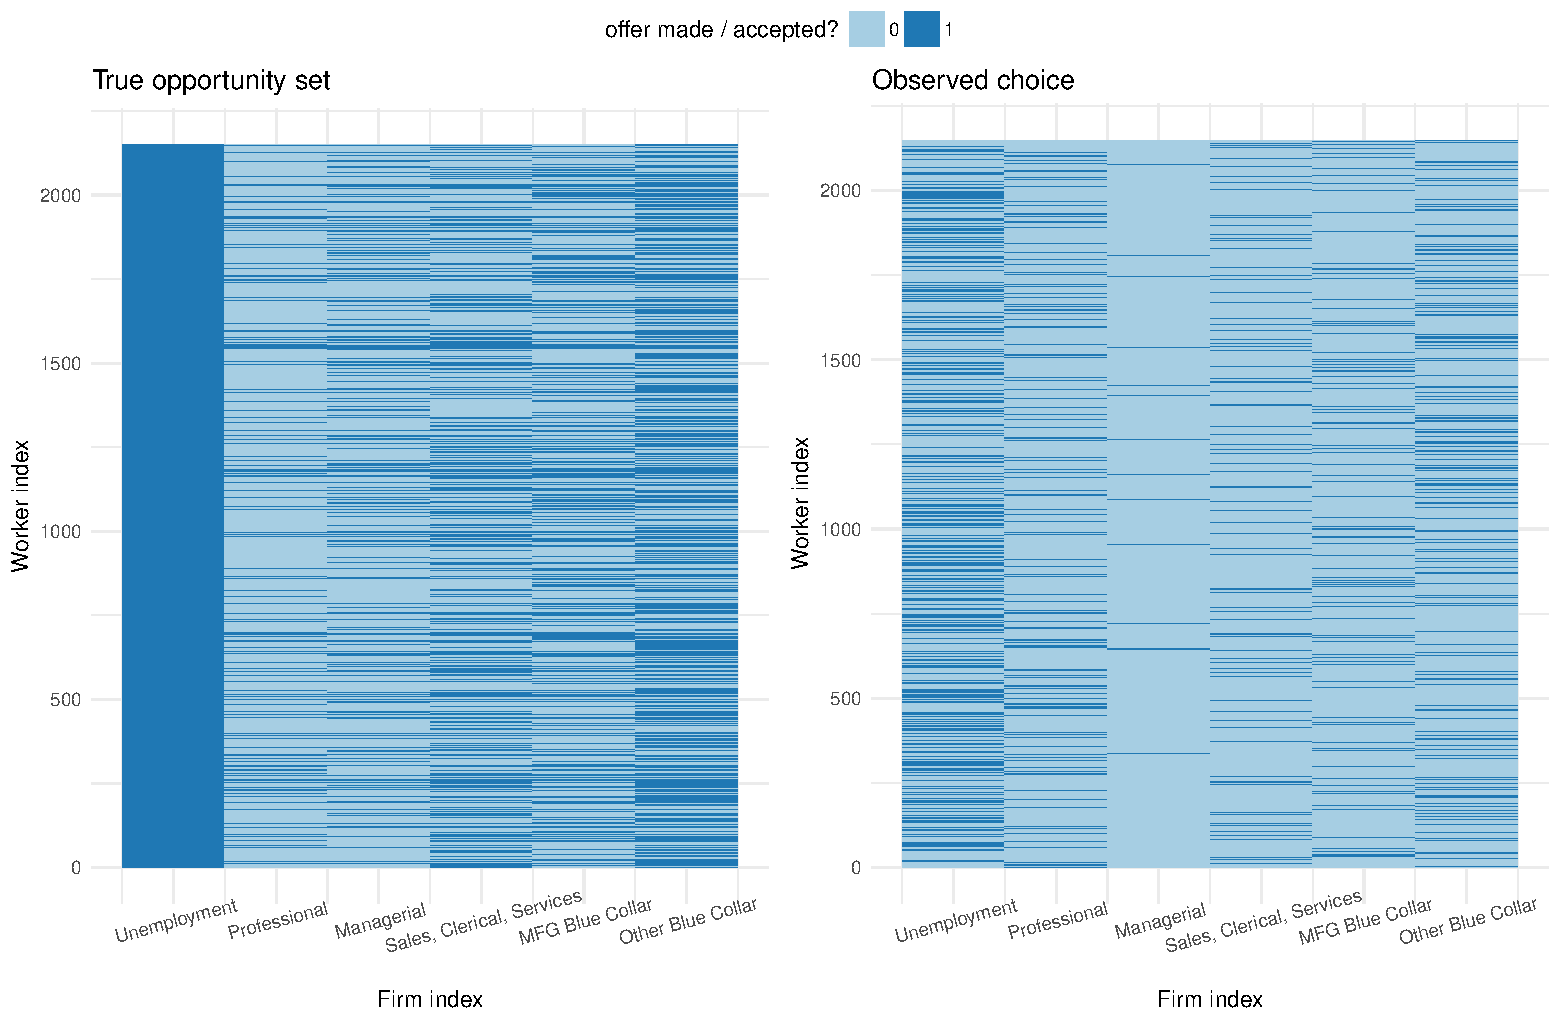
\includegraphics[width=\textwidth,keepaspectratio]{../figure/sim_labor_nojobs_trueopp_obschoice}
  \caption[True opportunity set vs observed choice.]{Binary heat map for the
    true opportunity set (left) and observed choice (right). A dark blue cell
    indicates that an offer was made (or accepted) between the firm in the
    corresponding column and the worker in the corresponding row.}
  \label{fig:sim_labor_nojobs_trueopp_obschoice}
\end{figure}

\section{Issues with MCMC convergence}
\label{sec:simulation_beta_opp_correlation}

A big reason for the poor mixing of firms' preference parameters $\beta$ is the
high correlation between $\beta$ and the opportunity set (Figure~\ref{fig:sim_labor_nojobs_opp_beta_correlation_managerial}). Intuitively, at any
point during the MCMC chain, we cannot propose a new opportunity set that is
very different from the current one because it would be too unlikely given the
current value of $\beta$. Likewise, we cannot propose too different a value for
$\beta$ because it would be rejected given the current opportunity set.

\begin{figure}[tbp]
  \centering
  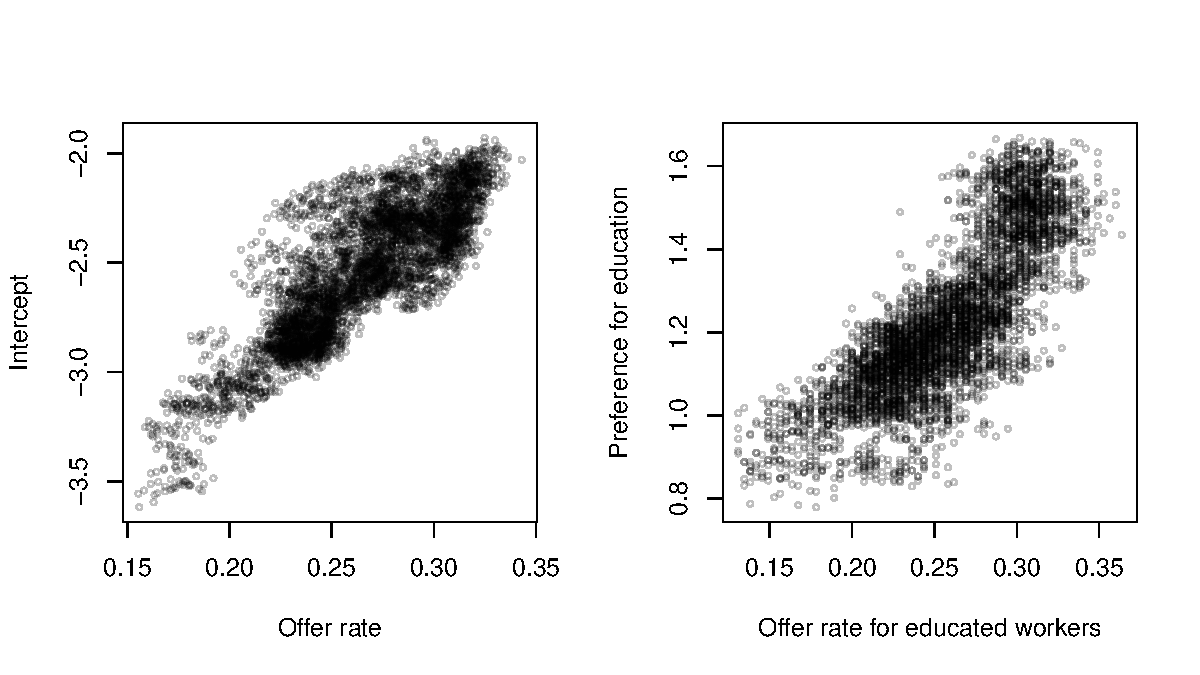
\includegraphics[width=\textwidth,keepaspectratio]{../figure/sim_labor_nojobs_opp_beta_correlation_managerial}
  \caption[Correlation between the opportunity set and $\beta$.]{Correlation
    between the opportunity set and $\beta$. The left panel shows the
    correlation between the $\beta$ intercept and the offer rate of a firm. When
  the intercept is high, the firm is also much more likely to extend an offer.
  The right panel shows the correlation between the $\beta$ for education and
  the offer rate for highly educated workers (top 25\% percentile). Once again,
  we see that if the $\beta$ for education is high, the firm is much  more
  likely to extend an offer to educated workers.}
  \label{fig:sim_labor_nojobs_opp_beta_correlation_managerial}
\end{figure}


This problem is especially severe for a firm with only a few workers. If we
propose a new opportunity set in which this firm extends the offer to a new
worker and this worker is very different from the current workers, then this new
offer will heavily affect the estimate for $\beta$. In contrast, for firms with
a large sample size, there is already a lot of information to precisely estimate
their preference. Making one new offer in these cases will not substantially
change the estimate.

Currently, I make random-walk proposals for $\beta$ and the opportunity set,
which insufficiently takes into account this correlation, causing poor mixing. A
potential solution to this problem is to make a correlated proposal for $\beta$
and for the opportunity set: if we propose a new $\beta$ that puts a high
emphasis on workers' education, then we should also perturb the opportunity set
to make more offers to highly-educated worker. While the concept is simple, this
approach is not straightforward to engineer, and is left for future
research.\footnote{Alternatively, we may reparameterize the model entirely and
  eliminate the opportunity set, whose binary nature makes it impossible to use
  more modern MCMC approaches such as Hamiltonian Monte Carlo. A potential
  alternative parameterization is \citet{Logan2008}'s, which samples directly
  from the utility space.}

\section{Estimation issues when the reservation choice is unobservable}
\label{sec:reservation_choice}

In Chapter~\ref{chap:FDI}, I will apply this two-sided matching model to the FDI
matching market, where countries extend offers to MNCs, and MNCs choose the best
country to invest among their set of options. However, an important difference
between the labor market and the FDI market is that in the latter we often will
not observe the ``reservation choice,'' i.e. the choice that will always be
available regardless of what the other side offers.\footnote{I call unemployment
  the ``reservation choice'' in reference to the ``reservation wage'' in game
  theory and economic models.} In the labor market, this ``reservation choice''
is unemployment. In the FDI market, it is staying in the home country and not
opening up a subsidiary abroad. Since most firm-level FDI data is collected by
surveying firms that have made an investment abroad, we are not observing the
firms who consider investing abroad but decide to stay put. Intuitively, we have
a sample selection problem where we only observe firms who have made it abroad.
This problem has different consequences depending on whether we are estimating
firms' preference or countries' preference. This section investigates how
missing this information affects the estimates of our model.

To imitate the FDI market data, at the end of the labor matching process I
remove all the unemployed workers, resulting in a sample of 1530 workers across
5 firms.

Figure~\ref{fig:sim_labor_nojobs_nounemp_alpha} shows that our estimates of
workers' preference are unaffected. This result makes sense---since we are still
observing 1530 workers choosing one firm over others, we still get a lot of
information about their preference. Not observing the workers who decide to stay
unemployed reduces our sample size, but otherwise does not pose any
problem.\footnote{In a sense, we avoid this problem by assuming that all workers
  have the same preference. Thus, even though we do not observe workers that are
  unemployed, there is still only one set of preference parameters and for all
  workers, which can be estimated from the workers that we do observe.}
Therefore, when applying the two-sided logit model to the FDI market, the
estimates for MNCs' preference will still be reliable.

\begin{figure}[tbp]
  \centering
  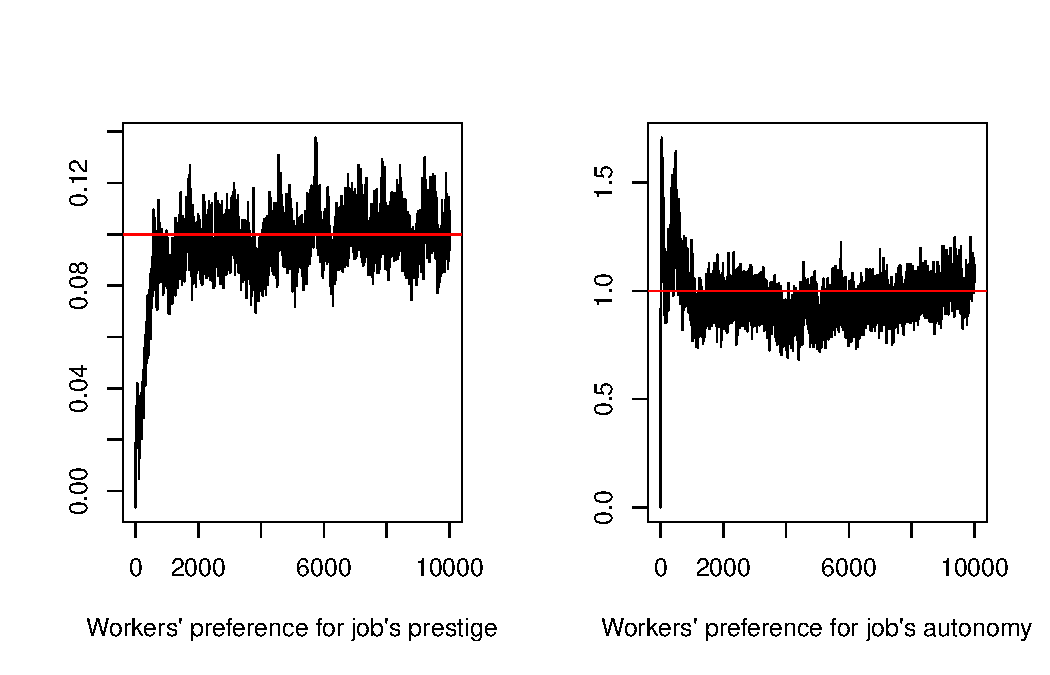
\includegraphics[width=\textwidth,keepaspectratio]{../figure/sim_labor_nojobs_nounemp_alpha}
  \caption[Estimates of workers' preference when the reservation choice is
  unobserved]{Estimates of workers' preference are unchanged even when we do not
    observe workers that choose unemployment (i.e., the reservation choice).}
  \label{fig:sim_labor_nojobs_nounemp_alpha}
\end{figure}

On the other hand, our estimates for firms' preference can have serious bias.
Figure~\ref{fig:sim_labor_nojobs_nounemp_managerial} shows the trace plots of
the preference of the managerial firm, which no longer overlaps with the true
values, indicated by the red line. The estimate of the rate at which the
managerial firm makes an offer is too high, as demonstrated both by the high
offer rate in the first panel and the high intercept term in the second
panel.\footnote{The firm makes an offer if the utility function is positive.
  Hence, if the intercept term is too high, the probability of this firm making
  an offer is also too high.}

This bias happens because we are only observing high quality workers, who
receive good enough offers that they decide to accept them instead of remaining
unemployed. Since our sample only include only these high quality workers, it
looks as if firms extend an offer to everyone, causing our model to think that
firms are more generous than they are. Therefore, the sampled intercept term
will be too high and the sampled opportunity set will have more offers than the
true opportunity set.

\begin{figure}[tbp]
  \centering
  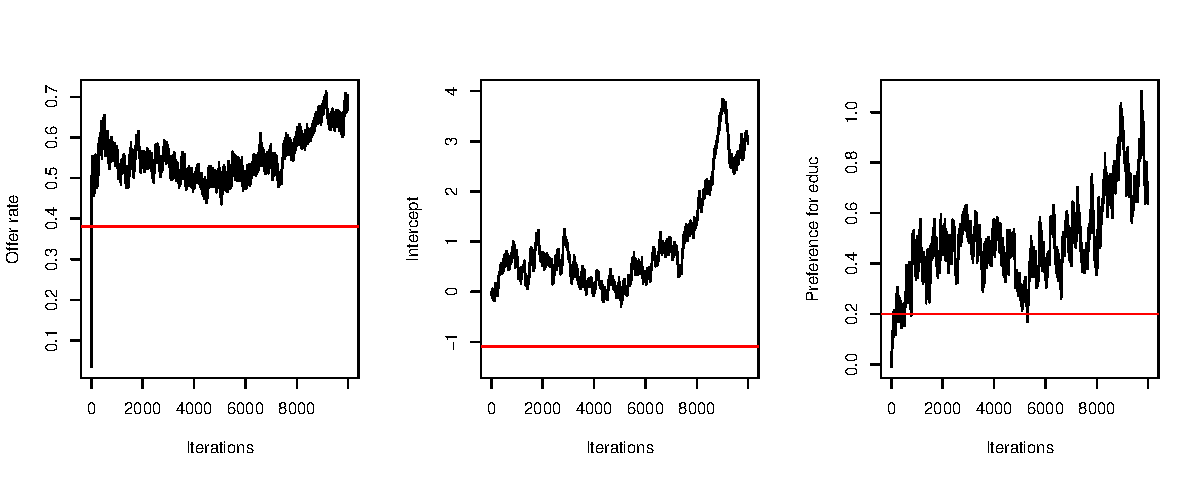
\includegraphics[width=\textwidth,keepaspectratio]{../figure/sim_labor_nojobs_nounemp_managerial}
  \caption[Estimates of firms' preference when the reservation choice is
  unobserved.]{Estimates of firms' preference are biased when we do not observe
    workers that choose unemployment (i.e. the reservation choice).}
  \label{fig:sim_labor_nojobs_nounemp_managerial}
\end{figure}

Another way to get the intuition around this problem is to consider how the
opportunity set is sampled. Whenever a good offer is proposed to be added in the
opportunity set, if we observe that the worker works work at a bad job, then it
is unlikely that the good offer was really made. Otherwise, the worker would
have taken it! This is how the sampling of the opportunity set avoids adding
spurious offers.

For this process to work well, unemployment needs to be an option so that we can
anchor other jobs against this bad option. Essentially, by observing a lot of
people who are unemployed, we know that other firms have not extended an offer
to these people, and thus allowing us to better estimate their preference. When
we do not observe the unemployed workers, we no longer have this information.
Therefore, our estimate are no longer accurate.

In sum, these findings have several implications. First, the estimate of the
workers' preference is unaffected. For the FDI market, this means that we can
still rely on the estimates of MNCs' preference without any change. Second,
given that we need a ``bad'' choice to anchor the estimate of firms' preference,
we can still rely on the estimates for the highly desirable firms. For these
firms, even without unemployment, there are still other worse firms to compare
to. Therefore, the estimates of their preference will still be accurate. For
example, conditional the estimated workers' preference, professional firm is the
most highly coveted job. Indeed
Figure~\ref{fig:sim_labor_nojobs_nounemp_offer_rate} shows the our estimates for
its parameters are still correct, unlike the estimate for other blue collar, a
much less desirable job. For the FDI market, this means that preference of
highly desirable countries are the most reliable, and others' less so.

\begin{figure}[tbp]
  \centering
  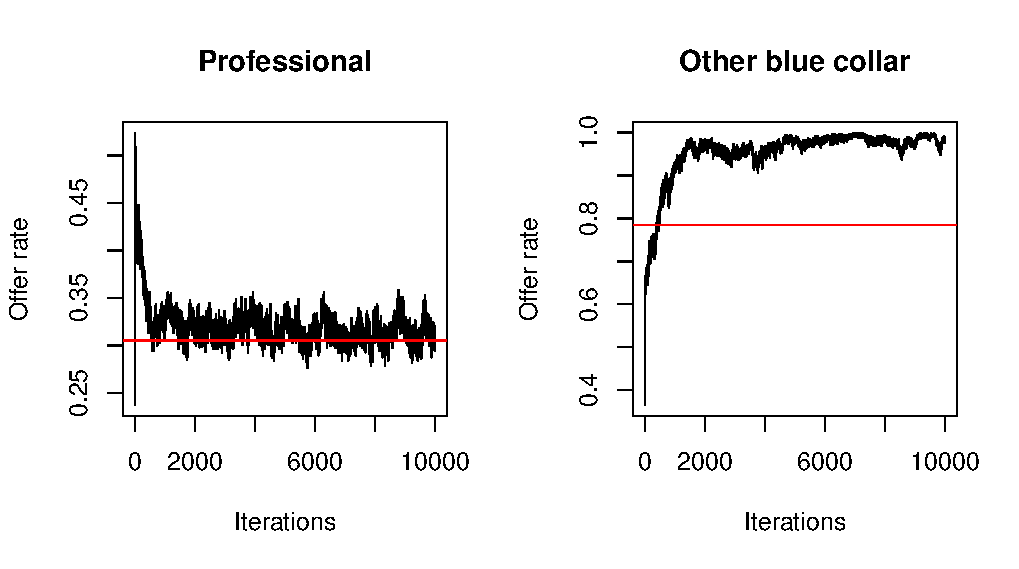
\includegraphics[width=\textwidth,keepaspectratio]{../figure/sim_labor_nojobs_nounemp_offer_rate}
  \caption[Estimates for the preference of a desirable and an undesirable firm.]{The estimates }
  \label{fig:sim_labor_nojobs_nounemp_offer_rate}
\end{figure}

\section{US labor market}
\label{sec:labor}

In this section I apply the two-sided logit model on the US labor market data, where the two sided logit model is originally developed for.

Services, professional, and managerial firms want highly educated workers. Blue
collar and MFG actually have a negative preference for highly educated workers,
perhaps because they consider these workers a flight risk, or a poor culture
fit.

We cannot compare the size of the estiamtes across firms, but we can compare
within firms. Interestingly, managerial firms seem to care more about age than
education, while professional firm care more about education than age.

In addition to interpretation at the utility space, we can also make prediction
in the normal space that is more interesting for policy formation. We can do the
log-odd interpretation, however better yet we draw Figure 4.2
show the probability of being hired for a typical worker. To produce this plot,
we simulate the firms' preference just like a logit model.

\begin{figure}[!ht]
  \centering
  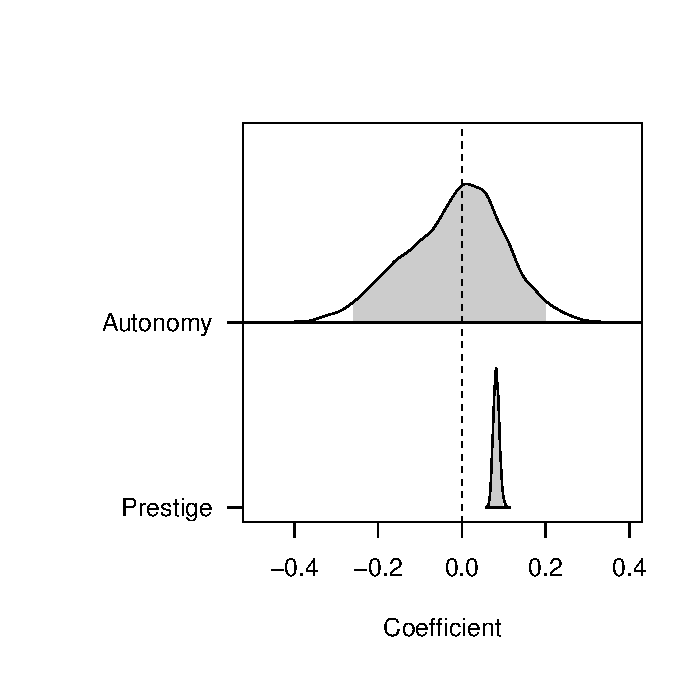
\includegraphics[width=0.75\textwidth,keepaspectratio]{../figure/labor_occ5_alpha}
  \caption[Workers' preference in the US labor market.]{Preference of workers for firms' characteristics. The density plot and the
    shaded region show the posterior distribution and the 95\% credible interval
    after burn-in. While prestige is highly valued by workers, autonomy seems to
    be less importance.}
  \label{fig:labor_occ5_alpha}
\end{figure}

\begin{figure}[!ht]
  \centering
  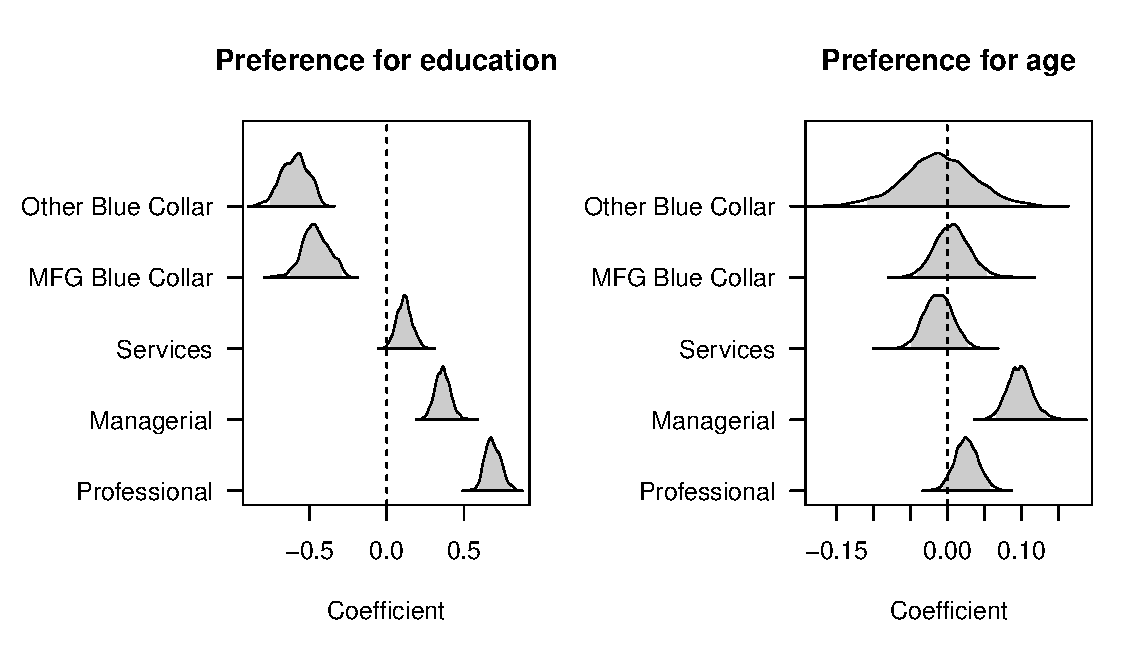
\includegraphics[width=\textwidth,keepaspectratio]{../figure/labor_occ5_beta_educ_age}
  \caption[Firms' preference in the US labor market]{Preference of firms for workers' education and
    age. Professional and managerial firms have a strong and positive preference
  for highly educated workers. While most firms do not highly value older workers,
  managerial firm stands out in their preference for age (likely as a
  proxy for experience).}
  \label{fig:labor_occ5_beta_educ_age}
\end{figure}

\begin{figure}[!ht]
  \centering 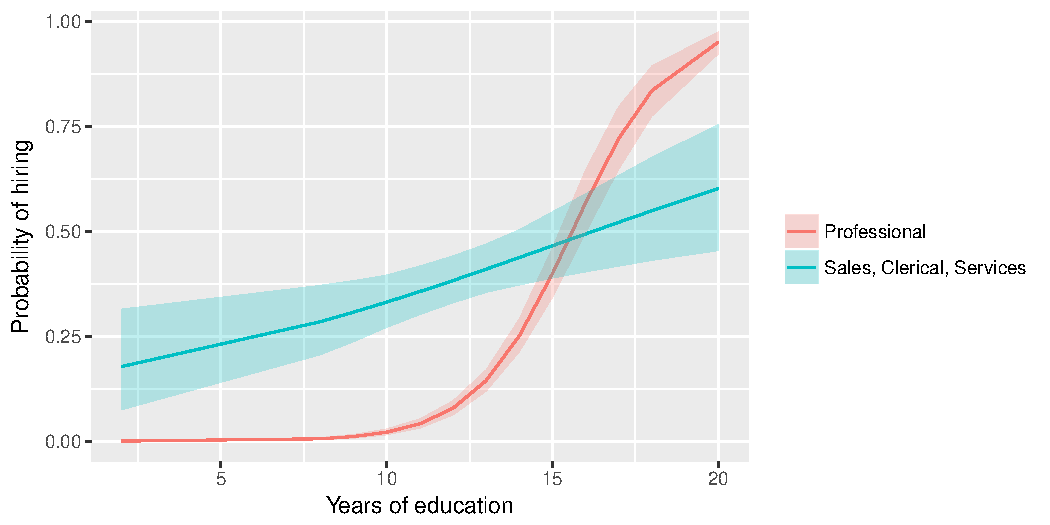
\includegraphics[width=\textwidth,keepaspectratio]{../figure/labor_occ5_educ_effect_on_hiring}
  \caption[The effect of education on the probability of a worker being hired in
  the US labor market.]{The
    effect of education on the probability of a worker being hired into a professional
    and a services job.}
  \label{fig:labor_occ5_educ_effect_on_hiring}
\end{figure}

\begin{figure}[!ht]
  \centering
  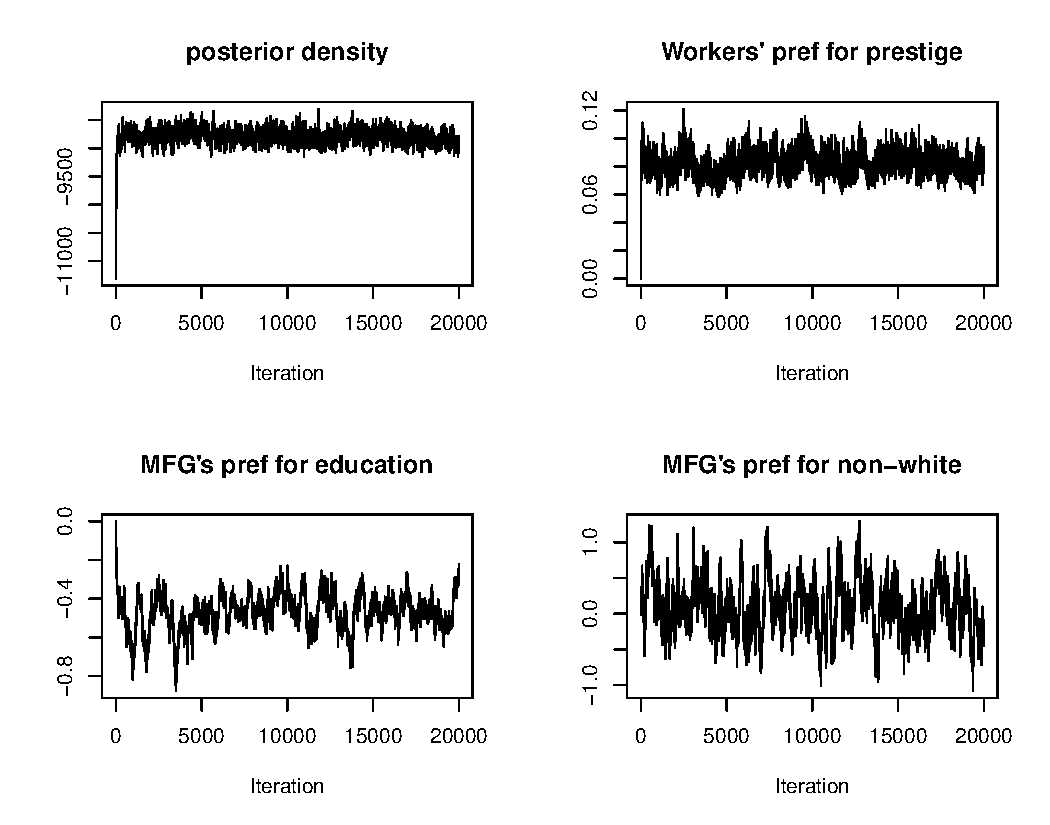
\includegraphics[width=\textwidth,keepaspectratio]{../figure/labor_occ5_misc_traceplots}
  \caption[Traceplots showing quick convergence for model of the US labor market.]{Trace plots of the posterior density and
    parameter samples, showing quick convergence.}
  \label{fig:labor_occ5_misc_traceplots}
\end{figure}
%%% Local Variables:
%%% mode: latex
%%% TeX-master: "AnhLe_dissertation.tex"
%%% End:
